\chapter{Effect of Lz4W \emph{rpoS} on \mbox{\emph{Escherichia coli}} promoters}

\section{Introduction}
\label{chap5:intro}

As discussed in the earlier chapters, \emph{rpoS} of Lz4W
(\emph{rpoS}\sub{Lz4W}) contains an amber mutation at codon 253 of
\emph{rpoS} reading frame. This is interesting from the view point
that several laboratory strains and natural isolates of \bact{Ec}
also harbor amber in
\emph{rpoS}~\citep{Jishage1997,Ivanova1992,Visick1997,Atlung2002}.
Furthermore, trehalose accumulation in these strains is dependent
on amber suppressor mutations~\citep{Rod1988}. Trehalose
accumulation in \bact{Ec} cells requires expression of
RpoS-controlled \emph{ots} gene~\citep{Hengge1991}. It is,
therefore, likely that amber suppression plays a crucial role in
expression of amber-mutated \emph{rpoS}\@. Moreover, these strains
exhibit variability in acid-sensitivity~\citep{Waterman1996}, and
in resistance to hydrostatic pressure \citep{Robey2001}. Similar
mutations in \emph{rpoS} have also been demonstrated in several
species of \emph{Salmonella}~\citep{Jorgensen2000,Sutton2000}.

Although, severely attenuated in RpoS-dependent stress-response,
many of these bacterial strains are not RpoS-null, even in the
absence of amber suppressor. There are several known mechanisms of
suppression of termination codon. Accumulating evidences indicate
that some of these even play regulatory roles in controlling gene
expression. Phenomena, such as, translational read-through,
frameshifting, and bypassing of the stop codon, occur even in
wild-type cells without any mutation in the translational
apparatus \citep{Hanna1996}. Su\-ch mechanisms play a very vital
role in bacteria (\emph{e.g.}, \emph{prfB} frameshifting in
\bact{Ec}), in viruses (\emph{e.g.}, capsid protein synthesis in
Q$\betaup$ phage) and have been proposed as a gene regulatory
mechanism in higher organism, such as, \emph{Drosophila}
\citep{Robinson1997}.

It has been demonstrated in earlier Chapters that the amber in
\lzsig{}, if not suppressed, would produce a $\sigmaup$, lacking
regions 4.1 and 4.2. Such a truncated \s{} would be intact upto
region 3.2. It is known that region 2 of $\sigmaup$\su{70} family
binds to $-$10 and region 4 binds to $-$35 elements of the
promoter. Remarkably, the region 4 of \siga{} in \bact{Ec} is
dispensable for promoters containing an \e{extended $-$10}
element~\citep[\seq{T\-G\-n\-T\-A\-T\-A\-A\-T},][]{Keilty1987,Kumar1993,Campbell2002}.
In fact, very recently, after elucidation of the crystal structure
of \emph{Thermus aquaticus} RNA polymerase, \citet{Campbell2002}
claimed that $\sigmaup$ region 1.2--3.1 contains all the elements
that are required for its function during transcription \e{in
vitro}.

In this Chapter, the ability of the \emph{rpoS}\sub{Lz4W} to
induce transcription from four known \emph{rpoS}-controlled
promoters of \bact{Ec} was examined. It was observed that \lzsig{}
in spite of lacking region 4, could activate a subset of promoters
in \emph{E. coli}. \lzsig{} was also tested for its ability to
complement catalase deficiency of a suppressor-containing
\bact{Ec} strain (JM101), where the indigenous \emph{rpoS} has
been mutated, to test the level to which suppressor tRNA can
suppress the amber mutation of \lzsig{}.

\section{Results}

Four known \emph{rpoS}-controlled promoters of \bact{Ec}, namely,
\emph{csiD}, \emph{bolAp1}, \emph{osmY}, and \emph{katE} were
tested by \emph{lacZ} genomic transcription fusion constructs. The
genomic copy of \emph{rpoS} in these strains was disrupted, and
the gene was provided on plasmid in \emph{trans}. To rule out any
inherent bias in cross-species complementation, \bact{Pa}
\emph{rpoS} (\emph{rpoS}\sub{Pa}) was taken as a positive control,
instead of native \bact{Ec} gene. All the complementation analyses
were carried out using high-copy-number plasmids. In case of
\lzsig{}, the plasmid vector was pBluescriptII KS+, and for
\emph{rpoS}\sub{Pa} it was pTZ18R. The effect of plasmid
copy-number, if any, was thought to be negligible by the fact that
both pBluescriptII KS+ and pTZ18R are high copy-number plasmids.
In plasmid p4C12 (contains \lzsig), the \emph{rpoS} was cloned in
the opposite direction to that of \emph{lacZ} promoter of the
vector to exclude its effect on the expression of \emph{rpoS}.


\subsection{Effect of Lz4W \emph{rpoS} on \emph{bolAp1}
promoter}

The \e{bolAp1} promoter in \bact{Ec} is regulated by \e{rpoS}. The
is responsible for the production of a \U{13}{kDa} morphogen in
the cell. To examine whether Lz4W \emph{rpoS} is capable of
activating \bact{Ec} \emph{bolAp1} promoter, p4C12 was introduced
into the strain ZK918~\citep[kind gift from R. Kolter. See
Table~\ref{ecolistrains} on page \pageref{ecolistrains} for
genotype]{Bohannon1991}. This strain was \emph{rpoS}-deficient due
to a deletional insertion generated by a \emph{rpoS}::Km fusion in
the genome. It also carried a chromosomal transcriptional fusion
of \emph{bolAp1} promoter to the \emph{lacZ}, at the \emph{bolA}
locus. Because \emph{bolAp1} promoter is \emph{rpoS} dependent,
the phenotype of the strain was reported to be RpoS\su{$-$}
LacZ\su{$-$} Km\su{r}~\citep{Bohannon1991,Ramos1998}. The
$\betaup$-galactosidase activities were measured in ZK918
containing p4C12 (\lzsig{}), ZK918 containing pDB18R (\pasig{};
positive control), and ZK918 containing pBluescriptII KS+ alone as
the negative control (Figure~\ref{chap5:zk918}).

\begin{figure}[tbp]
\begin{narrow}{-1in}{-1in}
\centering
\includegraphics{figures/chap5_zk918}
\end{narrow}
\caption[$\betaup$-galactosidase activity in transformed
ZK918]{$\betaup$-galactosidase activity in ZK918
(\emph{bolA}::\emph{lacZ} \emph{rpoS}) with growth phase, when
transformed with p4C12, containing Lz4W \emph{rpoS}. Plasmid
pDB18R, containing full-length \emph{rpoS} of \emph{P.
aeruginosa}, was taken as positive control and pBluescriptII KS+
was taken as plasmid control. X-axis shows the OD at 600 nm and
Y-axis shows $\betaup$-galactosidase activity in Miller units.}
\label{chap5:zk918}
\end{figure}

The $\betaup$-galactosidase activity of ZK918 containing p4C12 and
pDB18R were almost two-fold higher than the empty plasmid control,
along all the growth phases. While there was a peak of activity
for p4C12, at the early stationary phase (OD\sub{600} $\sim$1),
the activity decreased to the level observed in the presence of
\bact{Pa} \emph{rpoS} during the late stationary phase of growth.
This suggested that as shown in \bact{Ec}, the \e{bolAp1} promoter
is recognized and transcribed by both \lzsig{} and \pasig{} at the
stationary phase.

\subsection{Effect of Lz4W \emph{rpoS} on \emph{csiD} promoter}

The \e{csiD} is a carbon starvation induced gene in \bact{Ec} and
known be \e{rpoS}-controlled. The ability of \emph{rpoS}\sub{Lz4W}
to induce \emph{csiD} promoter was tested in the strain GJ2733
\citep[kind gift from J. Gowrishankar]{Rajkumari2001}, bearing an
operon fusion of \emph{csiD} promoter and \emph{lacZ}\@. The
indigenous \emph{rpoS} was disrupted in this strain by moving the
\emph{rpoS359}::Tn\emph{10} from RH90 \citep{Barth1995}. The
phenotype of the strain was reported to be LacZ\su{$-$},
RpoS\su{$-$}, Tc\su{r}~\citep{Rajkumari2001}. The production of
$\betaup$-galac\-to\-sidase was monitored in GJ2733 containing
\emph{rpoS}\sub{Lz4W} on p4C12, \pasig{} on pDB18R, and
pBluescriptII KS+ as empty plasmid control. There was a visible
difference of $\betaup$-galactosidase activities among these
strains on X-gal plate (Figure~\ref{chap5:csid_lacz}). The
$\betaup$-galactosidase activities of all these three strains were
also measured in LB broth in various growth phases
(Figure~\ref{chap5:csid_growth}). GJ2733 (p4C12) showed a marked
peak of $\betaup$-galac\-to\-sidase activity at late stationary
phase (OD\sub{600} $\sim$1.5). The activity increased from 30
units to 120 (Figure~\ref{chap5:csid_growth}B). The strain
containing plasmid pDB18R on the other hand showed a constant
level of expression at around 150 units throughout the growth
phases, as though the promoter remained at permanently derepressed
state of activation. The strain also grew very slowly than the
plasmid control and the strain containing p4C12
(Figure~\ref{chap5:csid_growth}A).

\begin{figure}[tbp]
\begin{narrow}{-1in}{-1in}
\centering
\includegraphics{figures/chap5_csid_lacz}
\end{narrow}
\caption[$\betaup$-galactosidase activity of GJ2733 on X-gal
plate]{$\betaup$-galactosidase activity of GJ2733 on X-gal plate
when transformed with p4C12 containing Lz4W \emph{rpoS}, pDB18R
containing \bact{Pa} \emph{rpoS} and pBluescriptII KS+.}
\label{chap5:csid_lacz}
\end{figure}





\begin{figure}[tbp]
\begin{narrow}{-1in}{-1in}
\centering
\includegraphics{figures/chap5_csid_lacz_graph}
\end{narrow}
\caption[$\betaup$-galatosidase activity in transformed
GJ2733]{$\betaup$-galactosidase activity in complemented GJ2733
(\emph{csiD}::\emph{lacZ} \emph{rpoS}) with growth phase, when
transformed with p4C12 containing Lz4W \emph{rpoS} ($\triangle$).
Plasmid pDB18R, containing full-length \emph{rpoS} of \bact{Pa}
($\medcirc$), was taken as positive control and pBluescriptII
KS+($\Box$) was taken as plasmid control. \textbf{(A)} The growth
of the 3 strains studied, represented as turbidity of the culture
measured as OD at \U{600}{nm}, plotted in Y-axis. X-axis shows the
time in hours. \textbf{(B)} $\betaup$-galactosidase activity,
measured as Miller units, plotted in Y-axis against OD at
\U{600}{nm} in X-axis.} \label{chap5:csid_growth}
\end{figure}

\subsection{Effect of Lz4W \emph{rpoS} on \emph{osmY}
promoter}

The \e{osmY} gene in \bact{Ec} is responsible for the production
of an osmotically induced periplasmic protein, and its promoter is
regulated by \e{rpoS}. The effect of \emph{rpoS}\sub{Lz4W} on
\bact{Ec} \emph{osmY} promoter was measured in GJ2734~\citep[kind
gift from J Gowrishankar]{Rajkumari2001}, which contains an operon
fusion of \emph{osmY} promoter and \emph{lacZ}. The indigenous
copy of \emph{rpoS} was mutated by moving
\emph{rpoS359}::Tn\emph{10} from RH90~\citep{Barth1995}. The
phenotype of the strain was reported to be RpoS\su{$-$},
LacZ\su{$-$} and Tc\su{r}. The strain was transformed with plasmid
p4C12 containing \emph{rpoS}\sub{Lz4W}, pDB18R, containing
\emph{rpoS}\sub{Pa} and pBluescriptII KS+ as empty plasmid
control. The result of the measured $\betaup$-galactosidase
activities at various phases of growth is shown in
Figure~\ref{chap5:osmy_growth}.

As shown in Figure~\ref{chap5:osmy_growth}A,
\emph{rpoS}\sub{Lz4W}-transformed GJ2734 grew slower than the same
strain containing \emph{rpoS}\sub{Pa} and empty plasmid. The
$\betaup$-galactosidase activities
(Figure~\ref{chap5:osmy_growth}B) remained essentially the same
throughout the growth phases (note the scale of Y-axis).

\begin{figure}[tbp]
\begin{narrow}{-1in}{-1in}
\centering
\includegraphics{figures/chap5_osmy_graph}
\end{narrow}
\caption[$\betaup$-galactosidase activity in complemented
GJ2734]{$\betaup$-galactosidase activity in complemented GJ2734
(\emph{osmY}::\emph{lacZ} \emph{rpoS}) with growth phase, when
transformed with p4C12 ($\medcirc$) containing Lz4W \emph{rpoS}\@.
Plasmid pDB18R ($\triangle$), containing \bact{Pa} \emph{rpoS} was
taken as a positive control and pBluescriptII KS+ ($\Box$) was
taken as plasmid control. \textbf{(A)} The growth of the three
strains studied, represented as turbidity of the culture measured
as OD at \U{600}{nm}, plotted in Y-axis. X-axis shows the time in
hours. \textbf{(B)} $\betaup$-galactosidase activity, measured as
Miller units plotted in Y-axis against OD at \U{600}{nm} in
X-axis.} \label{chap5:osmy_growth}
\end{figure}

\subsection{Effect of Lz4W \emph{rpoS} on \emph{katE}
promoter} \label{chap5:kate}

In a similar study on the effect of \emph{rpoS}\sub{Lz4W} on
\emph{katE} (encoding stationary phase specific catalase HPII)
promoter in \bact{Ec} it was found that there was no difference of
$\betaup$-galactosidase activities amongst strains harboring
p4C12, pDB18R, and pBluescriptII KS+. The activities were measured
in GJ2782~\citep[kind gift from J Gowrishankar]{Rajkumari2002},
which contains \emph{katE}::\emph{lacZ} fusion at the $\lambdaup$
integration site. The strain was derived from
RH100~\citep{Hengge1993}, where the \emph{nlpD}--\emph{rpoS}
region were deleted from the chromosome. The
\emph{katE}::\emph{lacZ} from strain KT1008EL~\citep{Tanaka1997}
was moved into RH100. The phenotype of the strain was reported to
be RpoS\su{$-$}, LacZ\su{$-$} and Km\su{r}. This strain, when
transformed with p4C12, pDB18R, and pBluescriptII KS+, the
$\betaup$-galactosidase activities in all these three remained
constant around 1--5 units throughout the growth phase (data not
shown). Surprisingly, even pDB18R failed to restore activity,
indicating that \emph{katE} is probably not recognized at all by
\bact{Pa} \emph{rpoS}.

\subsection{Effect of amber-suppressor \emph{supE} on Lz4W \emph{rpoS}}

The results of the \e{lacZ} expression studies described above
indicated that the \lzsig{} could probably transcribe from atleast
two of the four \sigs{}-controlled promoters in \bact{Ec}. To
examine whether this expression is due to to a suppression of the
amber, the stationary phase specific catalase activity was assayed
in an \bact{Ec} strain bearing a known suppressor (JM101).

%We wanted to find out whether the amber in \lzsig{} can be
%suppressed by a known suppressor in \bact{Ec}. We chose catalase
%as a marker. As discussed in Section~\ref{chap5:kate}, promoter of
%\emph{KatE}, coding for HPII catalase is not affected by
%\emph{rpoS}\sub{Lz4W}. We tested the ability of a background
%amber-suppressor to restore back the \emph{KatE} promoter activity
%by \emph{rpoS}\sub{Lz4W}.

In \emph{E. coli}, there are two catalases known. Catalase HPI,
coded by \emph{katG} and HPII, coded by \emph{katE}. There is now
considerable evidence that both these genes are controlled by
\emph{rpoS}\@. In RpoS\su{$-$} mutant, the catalase levels are
poor and the RpoS\su{$+$} and RpoS\su{$-$} strains can be easily
distinguished by a simple H\sub{2}O\sub{2} bubbling test, where
dropping of H\sub{2}O\sub{2} directly on a colony will from
bubbling due to break down of H\sub{2}O\sub{2} by cellular
catalase~\citep{Mulvey1988}.

JM101, which contained \emph{supE}, a known amber-suppressor, was
made RpoS\su{$-$} by P1 transduction, by moving
\emph{rpoS359}::Tn\emph{10} allele from Rh90 (see Sections
\ref{rh90_lysate} and \ref{P1_transduction} on page
\pageref{P1_transduction} for datails). The resulting strain
named, MJMRH is RpoS\su{$-$}, Catalase\su{$-$}, Tc\su{r} and
\emph{supE}\@. This strain was then transformed with plasmid p4C12
containing \emph{rpoS}\sub{Lz4W}, pDB18R containing
\emph{rpoS}\sub{Pa} as positive control, and pBluescriptII KS+ as
plasmid control. The H\sub{2}O\sub{2} bubbling test was performed
on these three strains (Figure~\ref{chap5:jm101}).

\begin{figure}[tbp]
\centering
\includegraphics{figures/chap5_jm101}
\caption[H\subsf{2}O\subsf{2} bubbling test on complemented
MJMRH]{H\subsf{2}O\subsf{2} bubbling test on MJMRH transformed
with p4C12 containing Lz4W \emph{rpoS}, pDB18R containing
\bact{Pa} \e{rpoS}, and pBluescriptII KS+ as plasmid control. The
transformed plasmid in each case is labelled on top.}
\label{chap5:jm101}
\end{figure}

MJMRH expectedly, had very little catalase activity when
transformed with empty plasmid (track marked as pBluescriptII KS+
in Figure~\ref{chap5:jm101}). Cells transformed with pDB\-18R
(track marked as pDB18R in Figure~\ref{chap5:jm101}) exhibited
very high activity. The activity was intermediate in cells
transformed with p4C12 (track marked as p4C12 in
Figure~\ref{chap5:jm101}). Although, pDB18R and p4C12 could not
activate transcription from \emph{katE} promoter, MJMRH showed a
marked increase in catalase activity, when transformed with
pDB18R. Possibly, both p4C12 and pDB18R induced transcription
through an unknown mechanism, through an indirect effect on
\emph{katE}, or by their effect on \emph{katG}, encoding HPI
catalase.

\subsection{Comparison of \emph{rpoS}-controlled promoters of
\bact{Ec}}

In an attempt to explain why \emph{csiD} and \emph{bolAp1}
promoters were activated by \lzsig{} while \emph{osmY} and
\emph{katE} remained unaffected, promoter sequences from 49
\bact{Ec} genes known to get transcribed by \sigs{}, were compared
(Figure~\ref{chap5:promoter_comparison}). Remarkably, both
\emph{csiD} and \emph{bolAp1} had \seq{G} at $-$14, whereas,
\emph{osmY} and \emph{katE} had \seq{T} and \seq{C}, respectively,
at this position. A search for \seq{G} at $-$14 of various
\sigs{}-controlled promoters in \bact{Ec} showed that it is
present only in \emph{ada}, \emph{dnaQp2}, \emph{dps},
\emph{galp1}, \emph{gor}, \emph{osmBp2}, \emph{pqi5p2},
\emph{proPp2}, \emph{rnaI}, \emph{topA}, and \emph{xthA} promoters
(underlined promoters in Figure~\ref{chap5:promoter_comparison}).
\seq{G} at $-$14 is known to enhance transcription both by \siga{}
and \sigs{} (see Section~\ref{chap5:discussion}). Moreover,
extended $-$10 promoters which are known to get transcribed by
\bact{Ec} \siga{} without region 4, has \seq{G} at $-$14. It is,
therefore, possible that \lzsig{} can activate transcription, in
spite of lacking region 4.

\begin{figure}
\centering
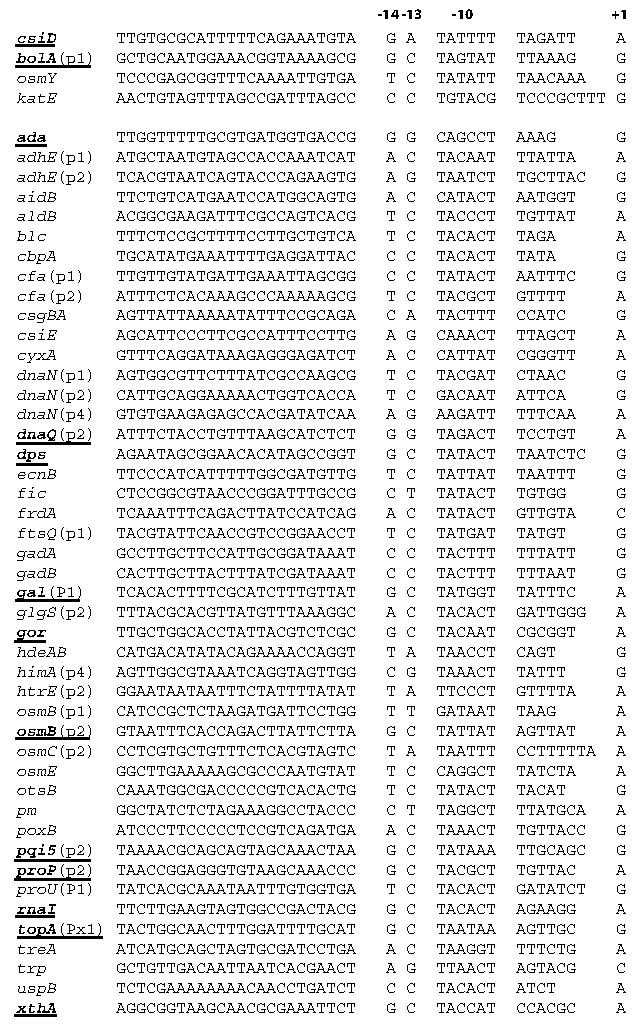
\includegraphics{figures/chap5_promoter_align}
\caption[Comparison of \emph{rpoS}-controlled promoter of \emph{E.
coli}]{Comparison of known \emph{rpoS}-controlled promoters of
\bact{Ec}. The sequences were gathered from various sources,
hand-aligned, and rearranged after \citet{Becker2001} to show
corresponding elements of promoters recognized by
$\sigmaup$\smallsu{70}. The promoters with G at position -14 are
underlined and in bold font. The transcription start site, $-$10,
$-$13, and $-$14 sites are indicated on top. The first four
promoters, separated from the rest by blank line, are tested in
this study.} \label{chap5:promoter_comparison}
\end{figure}


\section{Discussion}
\label{chap5:discussion}

The studies in this Chapter were carried out to examine whether
\lzsig{} could transcribe from known \bact{Ec}
\emph{rpoS}-con\-trolled promoters \e{in vivo}. Although, it
harbors an amber in its reading frame, \emph{rpoS}\sub{Lz4W} could
induce transcription from two (\emph{csiD} and \emph{bolAp1}) out
of four tested promoters.

There are contradictory reports regarding the ability of
\emph{Pseudomonas rpoS} to induce \bact{Ec} promoters. \bact{Pa}
\emph{rpoS} that was used in this study was reported to be able to
restore the catalase deficiency of \bact{Ec} \emph{rpoS}
mutant~\citep{Tanaka1994}. In a later study, however, the same
group could not detect any transcript of the same gene when
transformed in \bact{Ec}~\citep{Fujita1994}. In this study, it was
observed that \emph{rpoS}\sub{Pa} had marginal effect on
\emph{bolAp1} and no effect on \emph{osmY}\@. The \emph{csiD}
promoter, however, was activated by \pasig{} in all the growth
phases. The induction during the entry into stationary-phase, a
feature of \emph{rpoS}-controlled promoters, was distinctly
absent. It indeed restored the catalase activity in RpoS$^{-}$
cells, but obviously, not through a direct effect on
\emph{katE}\@. It also affected the growth rate of transformed
cells, but the effect was too variable to reach to any conclusion.

The pattern of induction by \lzsig{}, on the other hand,  shows
the characteristic peak of \emph{rpoS}-dependent \e{lacZ} activity
at the stationary phase for both \emph{bolAp1} and \emph{csiD}
promoters, even though it harbors an amber in the reading frame.
The induction was five folds for \emph{csiD} but only two folds
for \emph{bolAp1}. \emph{osmY} and \emph{katE} promoters were not
affected at all. As these promoters were not affected even by
\pasig{}, it is reasonable to state that \emph{Pseudomonas}
\emph{rpoS} can not activate \emph{osmY} and \emph{katE} promoters
of \bact{Ec}. Based on the results presented in this Chapter, it
can also be suggested that the amber in \lzsig{} is not
efficiently be suppressed by a known amber suppressor
(\emph{supE}) of \bact{Ec}.

The striking effect of \lzsig{} was observed on \emph{csiD}
promoter, where it activated the promoter almost to the level of
native \bact{Ec} gene. There could be two mechanisms by which
\lzsig{} could induce any promoter. First, the truncated protein
produced due to amber itself could be functional, or second, the
amber mutation is overcome by a read-through or by an
amber-suppression. Two strains where it induced transcription were
not reported to carry any amber suppressor; moreover, even
introduction of an exogenous suppressor allele could not
significantly restore its effect on transcription. Thus the
possibility of an suppressor mutation suppressing this amber was
less likely.

There is, however, exists a possibility that a read-through
full-length RpoS is produced which induced these promoters. The
existing data are not sufficient to discard this possibility.
There was an earlier report that the C-terminal 16 amino-acids are
important for \bact{Ec} RpoS activity on \emph{katE}, \emph{fic}
and \emph{bolA} promoters~\citep{Ohnuma2000}. In contrary, Lz4W
\emph{rpoS}, which lacks C-terminal entirely, could activate
\emph{bolA}, albeit, only two folds (Figure~\ref{chap5:zk918}).

Therefore, could it be possible that \lzsig{} is functional even
without region 4? In fact, it is now known that at least \siga{},
lacking region 4, can transcribe promoters with an \e{extended
$-$10}~\citep[\seq{T\-G\-n\-T\-A\-T\-A\-A\-T},][]{Keilty1987,Kumar1993,Campbell2002}\@.
\seq{TG} motif at $-$15 and $-$14 has been shown to be present in
25\% of all \bact{Ec} promoters~\citep{Burr2000}. Identical
mechanism could be operational for \sigs{}. The argument for this
possibility is threefold:

\begin{enumerate}

\item \siga{} and \sigs of \bact{Ec} are highly similar in their
recognition features at $-$10 of the promoters~\citep{Lee2001}.
Several \bact{Ec} promoters were found to be recognized by both
the $\sigmaup$ factors \emph{in
vitro}~\citep{Tanaka1993,Tanaka1995}. Selection experiments
(SELEX), performed \emph{in vitro} with \bact{Ec} \sigs{} selects
promoter sequence identical to that of \siga{}~\citep{Gaal2001}.
Both these $\sigmaup$ factors have almost identical sequences, in
the crucial functional regions~\citep{Lonetto1992,Gruber1997}.


\item Interaction between extended $-10$ with region 3.0 of
$\sigmaup$ has been well documented for both \siga{} and
\sigs{}~\citep{Voskuil1995,
Barne1997,Becker1999,Colland1999,Burr2000,Becker2001}.
Particularly important is \seq{G} at $-14$,  which has been shown
to have an activating effect on both \siga{}~\citep{Barne1997} and
\sigs{}~\citep{Becker2001}. We have also shown that both the
\lzsig{}-affected promoters, \emph{bolAp1} and \emph{csiD} have
\seq{G} at $-$14.

\item Moreover, experiments done with \emph{fic} promoter, which
does not use $-$35 contact at all~\citep{Tanaka1995}, and with
point mutations isolated in \emph{osmE}
promoter~\citep{Bordes2000}, as well as compilations of promoter
sequences~\citep{Espinosa1996} indicate that \sigs-dependent
promoters have weak or no $-$35 regions~\citep{Becker2001}.
Recognition of $-$35 element is, therefore, of less importance for
\sigs.

\end{enumerate}

It is, therefore, can be predicted that like \siga{}, \sigs{}
could function without region 4 for promoters with extended $-$10.
And it is probable that \lzsig{} can activate promoter with
extended $-$10 in spite of lacking region 4. It has been shown
that only a subset of \emph{rpoS}-controlled promoters that has
\seq{G} at $-$14 are potential candidate to get affected by
\lzsig{}, resulting in promoter discrimination within \emph{rpoS}
regulon. The implication of such discrimination, if at all
operational in Lz4W, remains to be investigated.\ding{45}
